\section{Method}
\usetikzlibrary{positioning}
\lstset{style=CStyle}

\subsection{Data Modeling}

\subsubsection{Query-Driven Design Analysis}
The database design is driven by the concrete read/write operations that the learning assistant must support.

\textbf{Primary write operations (ingestion and indexing):}
\begin{itemize}
    \item \textbf{Ingest document:} convert input files to text (MarkItDown/PDF processor), then create ordered text chunks with overlap.
    \item \textbf{Extract entities:} for each chunk, extract entity candidates with attributes (type, description) and attach provenance (chunk ID, file path).
    \item \textbf{Extract relations:} for each chunk, extract relationships between entities with keywords, description, and an initial weight.
    \item \textbf{Merge into the graph:} upsert entities and relationships, merging duplicated names and accumulating edge weights across multiple mentions.
\end{itemize}

\textbf{Primary read operations (retrieval for answering):}
\begin{itemize}
    \item \textbf{Keyword search:} find entities whose names/descriptions match query terms.
    \item \textbf{Local retrieval:} expand a bounded neighborhood (1--2 hops) from seed entities to gather precise facts.
    \item \textbf{Global retrieval:} retrieve broader sets of entities matching high-level themes.
    \item \textbf{Hybrid retrieval:} combine local and global candidate sets.
    \item \textbf{Path finding:} find multi-hop paths between two entities (for explainability and multi-hop reasoning).
    \item \textbf{Graph statistics:} compute density, degree distribution, and ``most connected'' entities to monitor graph health.
\end{itemize}

\subsubsection{Graph Data Model (Neo4j-Style Property Graph)}
We use a \textbf{property graph} model. This report presents the model in Neo4j terminology (labels, properties, relationships). The current prototype stores the graph in-memory (Python dictionaries), but the data model is directly portable to Neo4j.

\begin{table}[h]
\centering
\begin{tabular}{|p{3.1cm}|p{3.0cm}|p{7.2cm}|}
\hline
\textbf{Element} & \textbf{Type} & \textbf{Properties (examples)} \\
\hline
\texttt{:Entity} & Node label & \texttt{entity\_id} (unique), \texttt{entity\_type}, \texttt{description}, \texttt{created\_at}, \texttt{source\_ids[]} (chunk IDs), \texttt{file\_paths[]} \\
\hline
\texttt{:Chunk} & Node label & \texttt{chunk\_id} (unique), \texttt{content}, \texttt{tokens}, \texttt{chunk\_order\_index}, \texttt{file\_path} \\
\hline
\texttt{:RELATED\_TO} & Relationship & \texttt{description}, \texttt{keywords}, \texttt{weight}, \texttt{created\_at}, \texttt{source\_ids[]}, \texttt{file\_paths[]} \\
\hline
\texttt{:MENTIONED\_IN} & Relationship & Connects \texttt{:Entity}$\rightarrow$\texttt{:Chunk} to represent provenance explicitly (optional; prototype stores provenance as arrays). \\
\hline
\end{tabular}
\caption{Graph data model used by RAG\_Core (Neo4j-compatible).}
\end{table}

\begin{figure}[h]
\centering
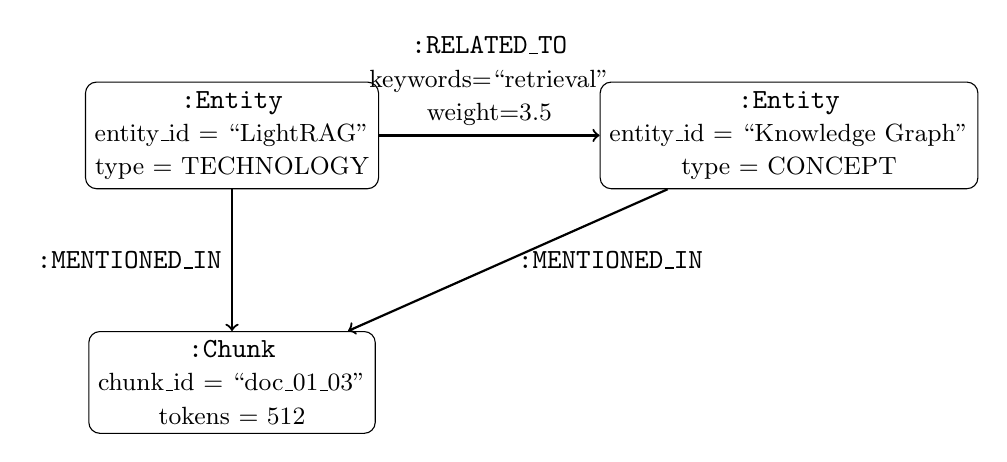
\begin{tikzpicture}[
  node distance=18mm,
  box/.style={draw, rounded corners, align=center, minimum width=35mm, minimum height=12mm},
    rel/.style={->, thick}
]
\node[box] (e1) {\texttt{:Entity}\\\small entity\_id = ``LightRAG''\\\small type = TECHNOLOGY};
\node[box, right=28mm of e1] (e2) {\texttt{:Entity}\\\small entity\_id = ``Knowledge Graph''\\\small type = CONCEPT};
\node[box, below=18mm of e1] (c1) {\texttt{:Chunk}\\\small chunk\_id = ``doc\_01\_03''\\\small tokens = 512};

\draw[rel] (e1) -- node[above, align=center]{\texttt{:RELATED\_TO}\\\small keywords=``retrieval''\\\small weight=3.5} (e2);
\draw[rel] (e1) -- node[left]{\texttt{:MENTIONED\_IN}} (c1);
\draw[rel] (e2) -- node[right]{\texttt{:MENTIONED\_IN}} (c1);
\end{tikzpicture}
\caption{Illustration of the property graph: entities as nodes; relations as edges; chunks for provenance.}
\end{figure}

\subsection{Implementation \& DB-Specific Queries}

\subsubsection{System Architecture}
The system follows a simple Frontend$\rightarrow$Backend$\rightarrow$Database pipeline. The ``database'' is the property graph (in-memory for the prototype; Neo4j-compatible for persistence). LLM calls are served via Ollama (general model for extraction/answering; dedicated translation model for VN$\leftrightarrow$EN).

\begin{figure}[h]
\centering
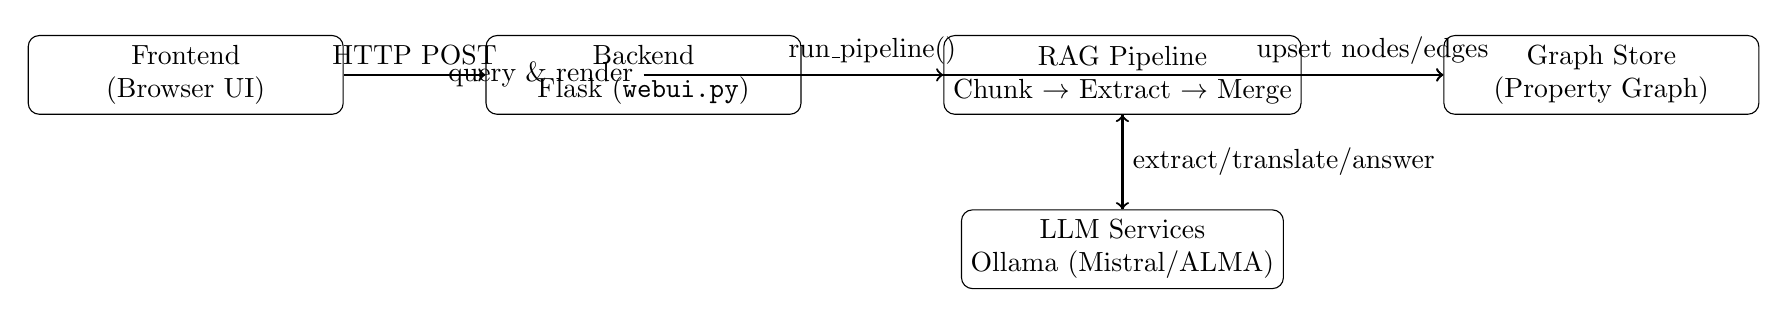
\begin{tikzpicture}[
  node distance=14mm,
  box/.style={draw, rounded corners, align=center, minimum width=40mm, minimum height=10mm},
    arr/.style={->, thick}
]
\node[box] (ui) {Frontend\\(Browser UI)};
\node[box, right=18mm of ui] (api) {Backend\\Flask (\texttt{webui.py})};
\node[box, right=18mm of api] (pipe) {RAG Pipeline\\Chunk $\rightarrow$ Extract $\rightarrow$ Merge};
\node[box, right=18mm of pipe] (db) {Graph Store\\(Property Graph)};
\node[box, below=12mm of pipe] (llm) {LLM Services\\Ollama (Mistral/ALMA)};

\draw[arr] (ui) -- node[above]{HTTP POST} (api);
\draw[arr] (api) -- node[above]{run\_pipeline()} (pipe);
\draw[arr] (pipe) -- node[above]{upsert nodes/edges} (db);
\draw[arr] (api) |- node[pos=0.25, left]{query \& render} (db);
\draw[arr] (pipe) -- node[right]{extract/translate/answer} (llm);
\draw[arr] (llm) -- (pipe);
\end{tikzpicture}
\caption{End-to-end architecture: UI to backend to graph store (Neo4j-compatible model).}
\end{figure}

\subsubsection{Core Code / Query Snippets}
To highlight graph-database-oriented querying, we extract a few focused snippets (not the whole codebase).

\textbf{(1) Graph upsert + merge (entity merge with provenance).}
\begin{lstlisting}[language=Python]
# GraphBuilder._merge_entity (simplified)
if entity_name in self.nodes:
    node = self.nodes[entity_name]
    node.description = merge(node.description, [e.description for e in entities])
    node.source_ids = union(node.source_ids, [e.source_id for e in entities])
    node.file_paths = union(node.file_paths, [e.file_path for e in entities])
else:
    self.nodes[entity_name] = GraphNode(
        entity_id=entity_name,
        entity_type=entities[0].type,
        description=merge_descriptions([e.description for e in entities]),
        source_ids=[e.source_id for e in entities],
        file_paths=[e.file_path for e in entities],
    )
\end{lstlisting}

\textbf{(2) Depth-limited neighborhood traversal (local retrieval).}
\begin{lstlisting}[language=Python]
# QueryEngine.entity_search (BFS, depth-limited)
to_visit = [(entity_id, 0)]
visited = set()
while to_visit:
    current, depth = to_visit.pop(0)
    if current in visited:
        continue
    visited.add(current)
    if depth < max_depth:
        for (u, v), edge in self.edges.items():
            if u == current and v not in visited:
                to_visit.append((v, depth + 1))
            elif v == current and u not in visited:
                to_visit.append((u, depth + 1))
\end{lstlisting}

\textbf{(3) Neo4j/Cypher equivalents (production-ready backend).}
\begin{lstlisting}[language=SQL]
// Full-text keyword search over Entity name + description
CALL db.index.fulltext.queryNodes('entityTextIndex', $q) YIELD node, score
RETURN node.entity_id, score ORDER BY score DESC LIMIT $k;

// 1-2 hop neighborhood expansion (undirected traversal)
MATCH (e:Entity {entity_id:$seed})-[r:RELATED_TO*1..2]-(n:Entity)
RETURN e, r, n;

// Multi-hop path finding (bounded)
MATCH p=(a:Entity {entity_id:$src})-[:RELATED_TO*1..3]-(b:Entity {entity_id:$tgt})
RETURN p LIMIT 5;
\end{lstlisting}

\subsection{Advanced Features Implementation}
Beyond basic graph storage and traversal, the system includes advanced features relevant to modern database applications:
\begin{itemize}
    \item \textbf{Hybrid query modes:} \texttt{naive/local/global/hybrid} retrieval modes (configurable) to trade off precision vs. coverage.
    \item \textbf{Bilingual query support:} optional Vietnamese$\leftrightarrow$English translation using a dedicated LLM client (ALMA-13B) before/after retrieval.
    \item \textbf{Structured context assembly:} retrieval results are formatted as JSON blocks (entities, relations, chunks) to reduce prompt ambiguity and improve answer grounding.
    \item \textbf{Graph provenance tracking:} nodes/edges store \texttt{source\_ids} and \texttt{file\_paths} to support traceability from answers back to document chunks.
    \item \textbf{Accuracy benchmarking bridge:} an integration module compares RAG\_Core outputs to LightRAG for validation in controlled tests.
\end{itemize}